\documentclass{article}
\usepackage{amsmath}
\usepackage{graphicx}
\begin{document}
\author{Ana Bhattacharjee}
\title{Equation of a Circle: Question 5}
\date{\today}
\maketitle{}

\begin{center}
  \begin{align}
    A = (-1, 1) \\
    (-1 - 3)^2 + 1^2 = 17 \\
    17 < 49
  \end{align}
  \par
  Point A is inside the circle.
  \par
  \begin{align}
    B = (10, 0) \\
    (10 - 3)^2 + (0)^2 = 49 \\
    49 = 49
  \end{align}
  \par
  Point B is on the circle.
  \par
  \begin{align}
    C = (4, -8) \\
    (4 - 3)^2 + (-8)^2 = 65 \\
    65 > 49
  \end{align}
  \par
  Point C is outside the circle.
\end{center}
You can also see the points visually on the graph below. 
\begin{figure}
  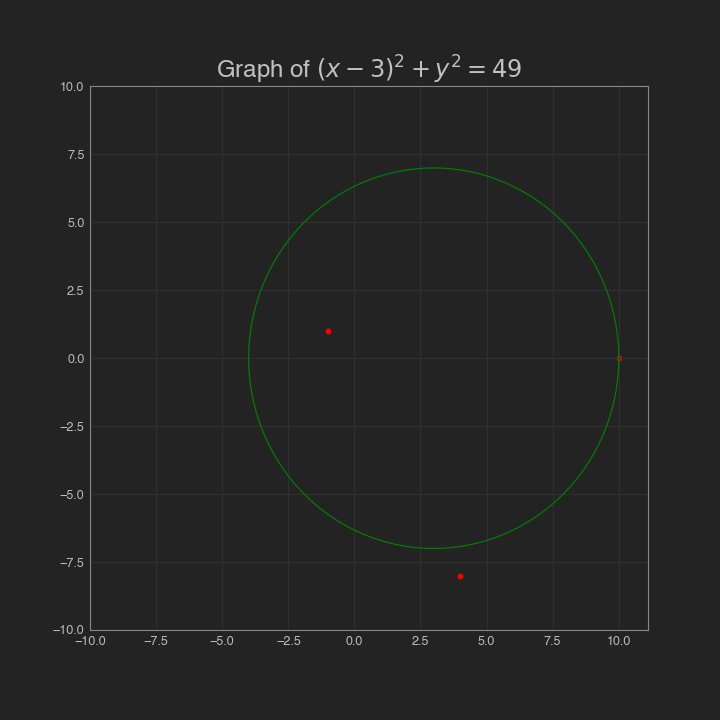
\includegraphics[width=1.2\columnwidth]{../../../../../../math/anna/geometry/coordinate_geometry/circles/q5/graph.png}
  \caption{Graph of Circle}
\end{figure}
\end{document}
